\newcommand{\makeNAMEFig}{%
\begin{figure}[!htbp]
    \centering
    \includegraphics[width=\linewidth]{figures/NAME}
    \caption{CAPTION}
    \label{fig:NAME}
\end{figure}
}


\newcommand{\makeSampleFig}{%
\begin{figure}[tb]
 \centering % avoid the use of \begin{center}...\end{center} and use \centering instead (more compact)
 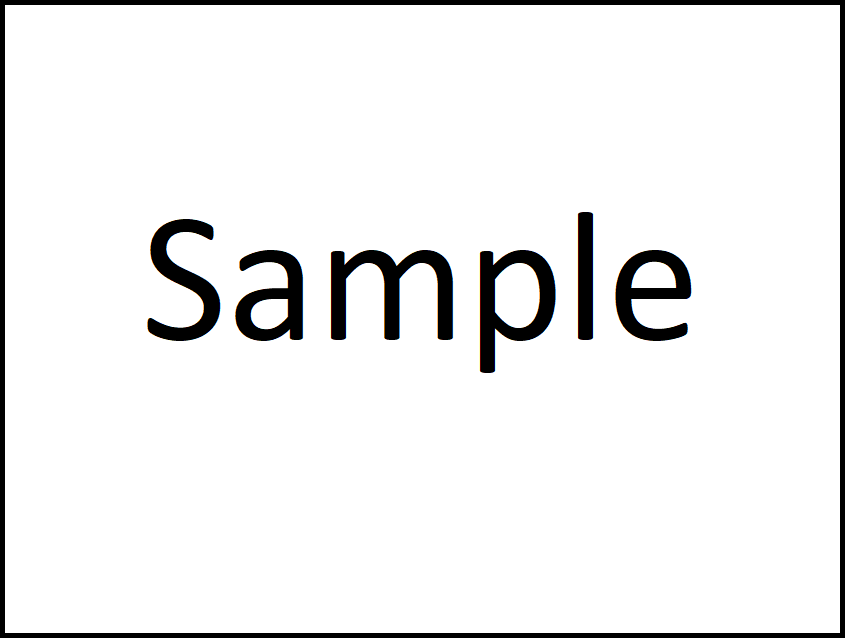
\includegraphics[width=\columnwidth]{sample}
 \caption{A visualization of the 1990--2015 data from \autoref{tab:vis_papers}. The image is from \cite{Isenberg:2017:VMC} and is in the public domain.}
 \label{fig:sample}
\end{figure}}

\newcommand{\makeSampleSegFig}{%
\begin{figure}[!htbp]
    \centering
    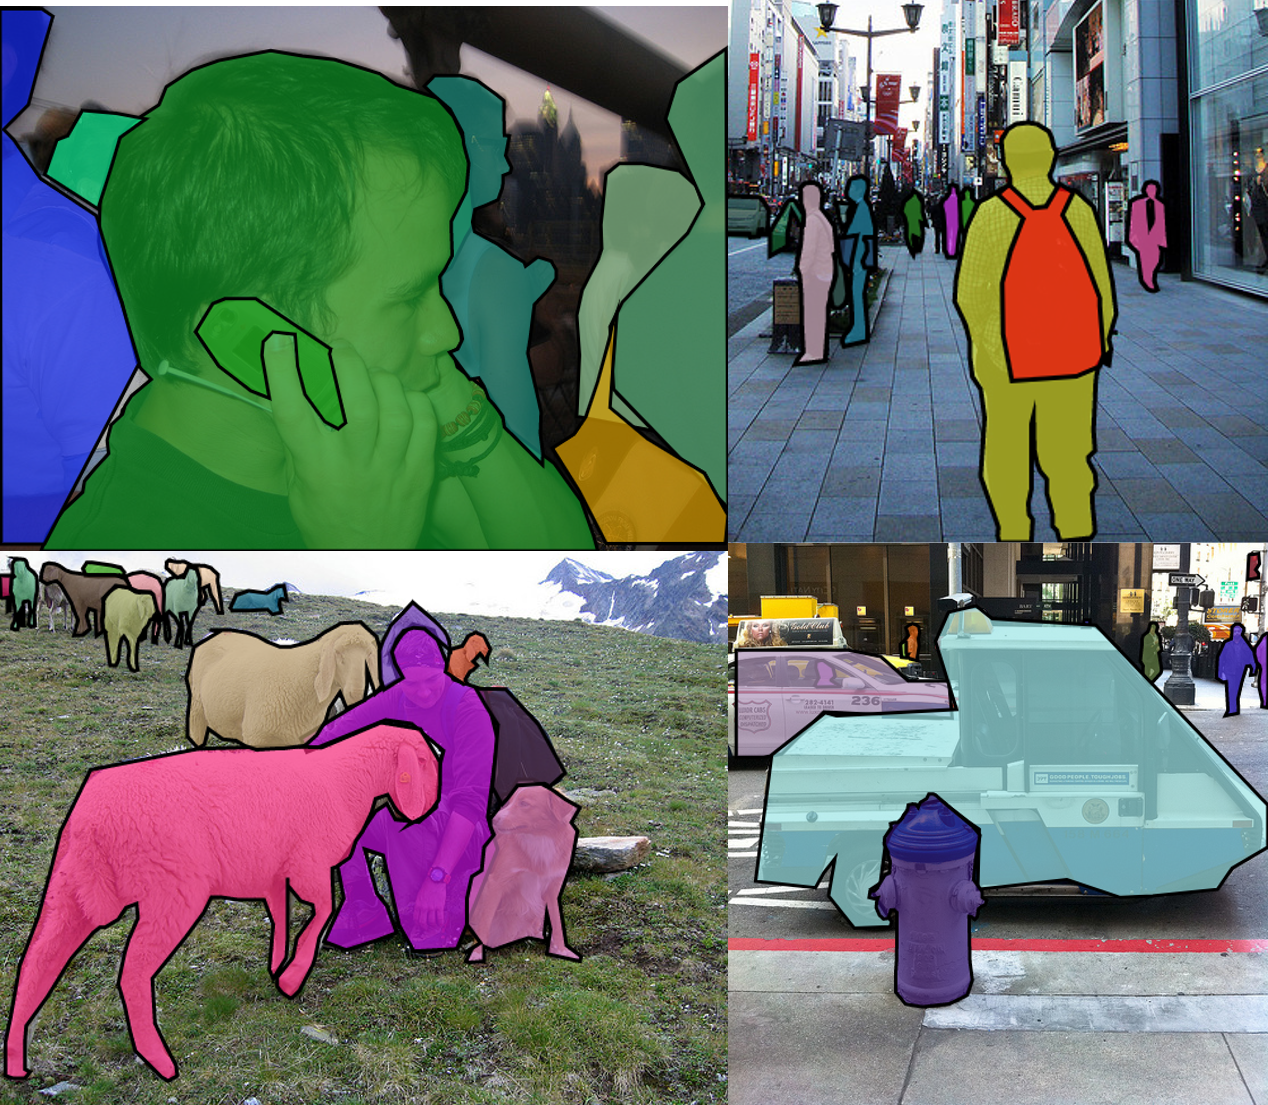
\includegraphics[width=\linewidth]{figures/sampleSegData}
    \caption{Common use cases for semantic segmentation involve relatively few foreground objects, low-resolution data, and limited complexity per object. Images retrieved from \url{https://cocodataset.org/\#explore}.}
    \label{fig:sampleSegData}
\end{figure}
}

\newcommand{\makeBeesFig}{%
\begin{figure}[!htbp]
    \centering
    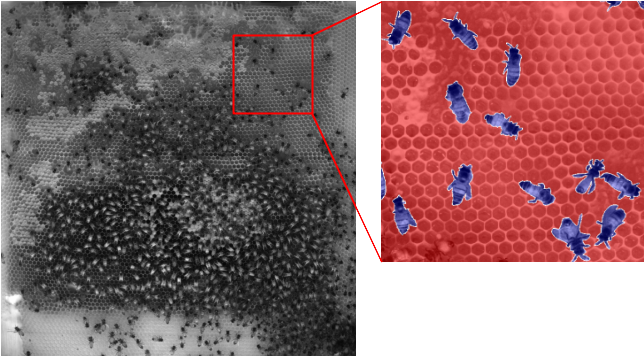
\includegraphics[width=\linewidth]{figures/bees}
    \caption{Sample segmentation involving a high-resolution image with many regions of interest and high foreground complexity. In such cases, unaided human annotation is infeasible with any time constraints. Image retrieved from \url{https://www.kaggle.com/kport354041/honeybee-positions}.}
    \label{fig:bees}
\end{figure}
}

\newcommand{\makeReconfigFigs}{%
\begin{figure*}[!htbp]
    \centering
    \subfloat[Example using component ID (the default) as a coloring label]{%
        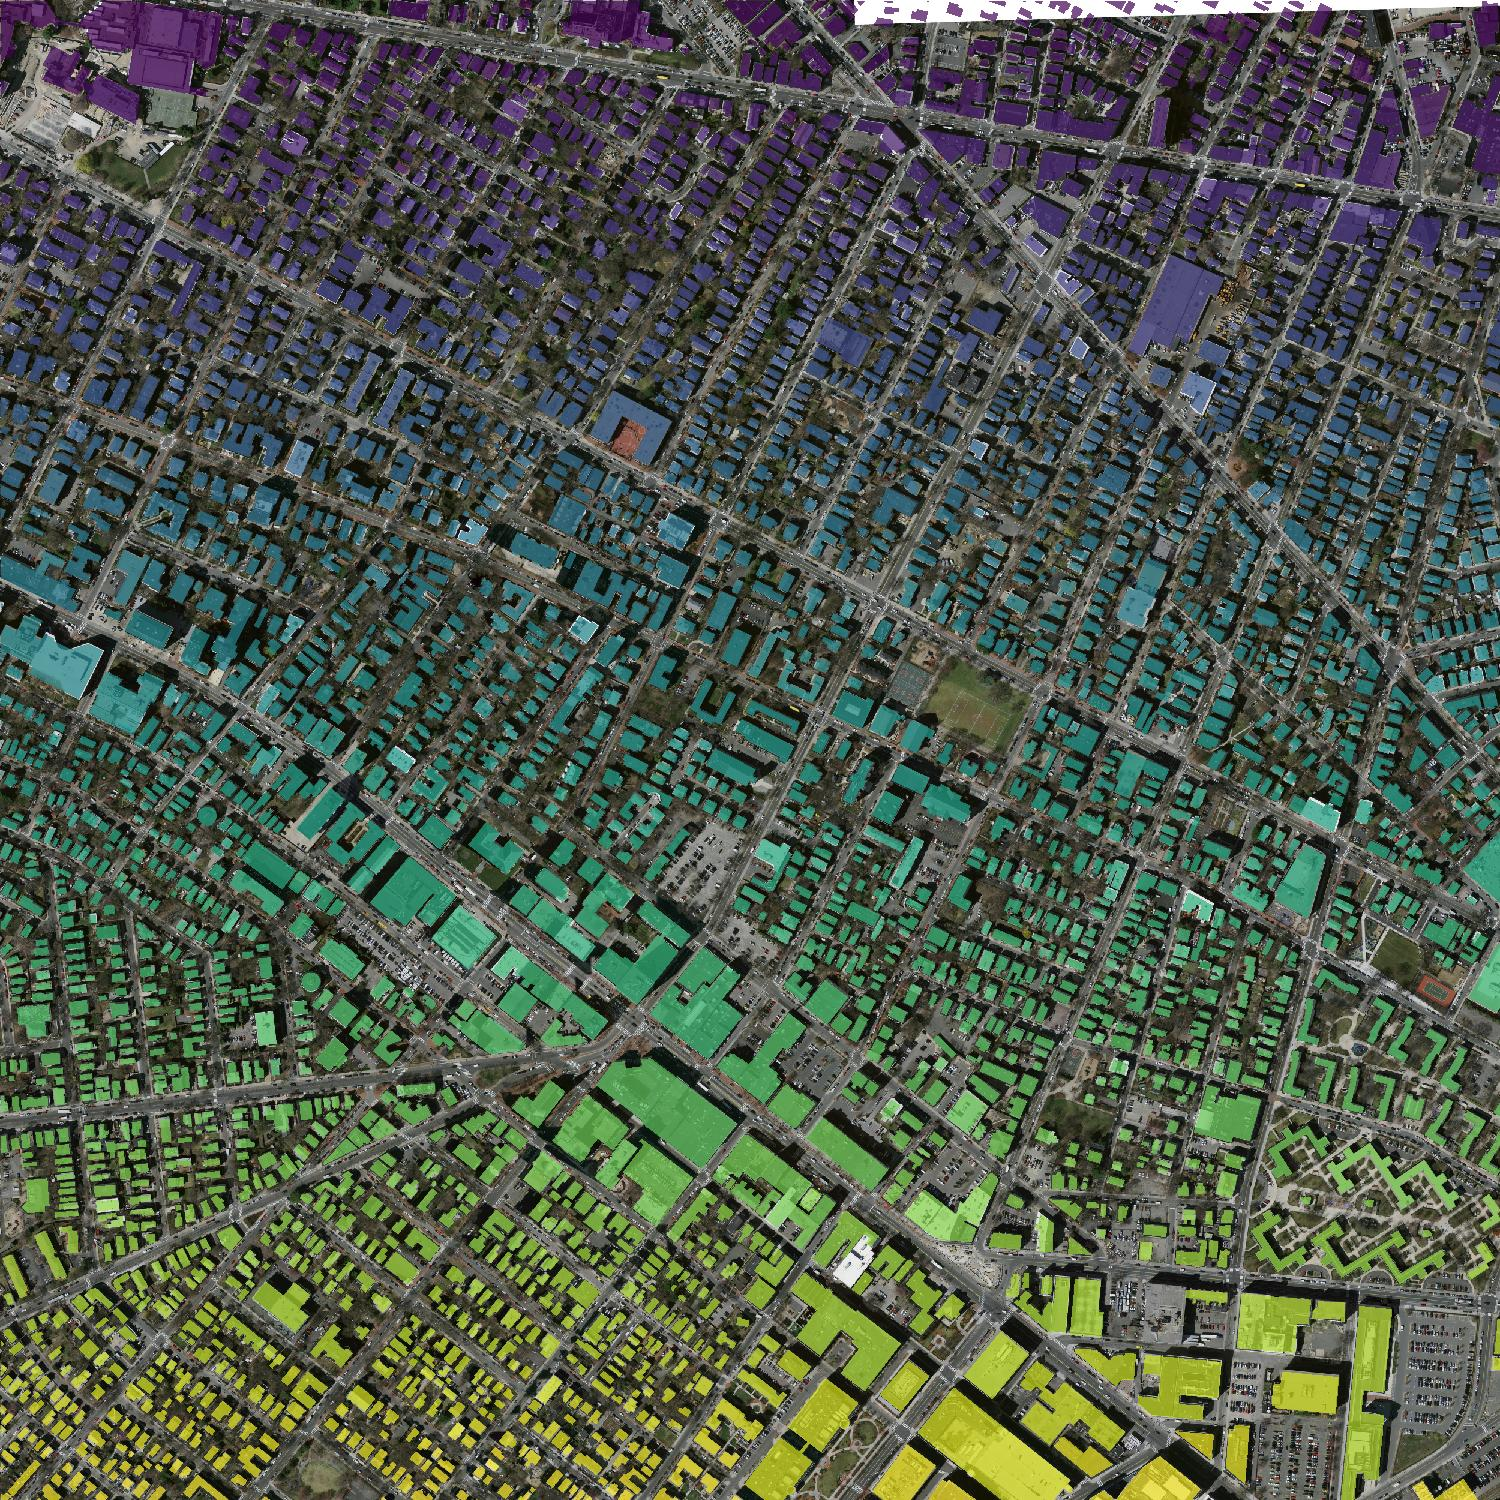
\includegraphics[width=0.25\linewidth]{figures/labelById}%
    }
    \hspace{1em}
    \subfloat[Example using component class as a coloring label]{%
        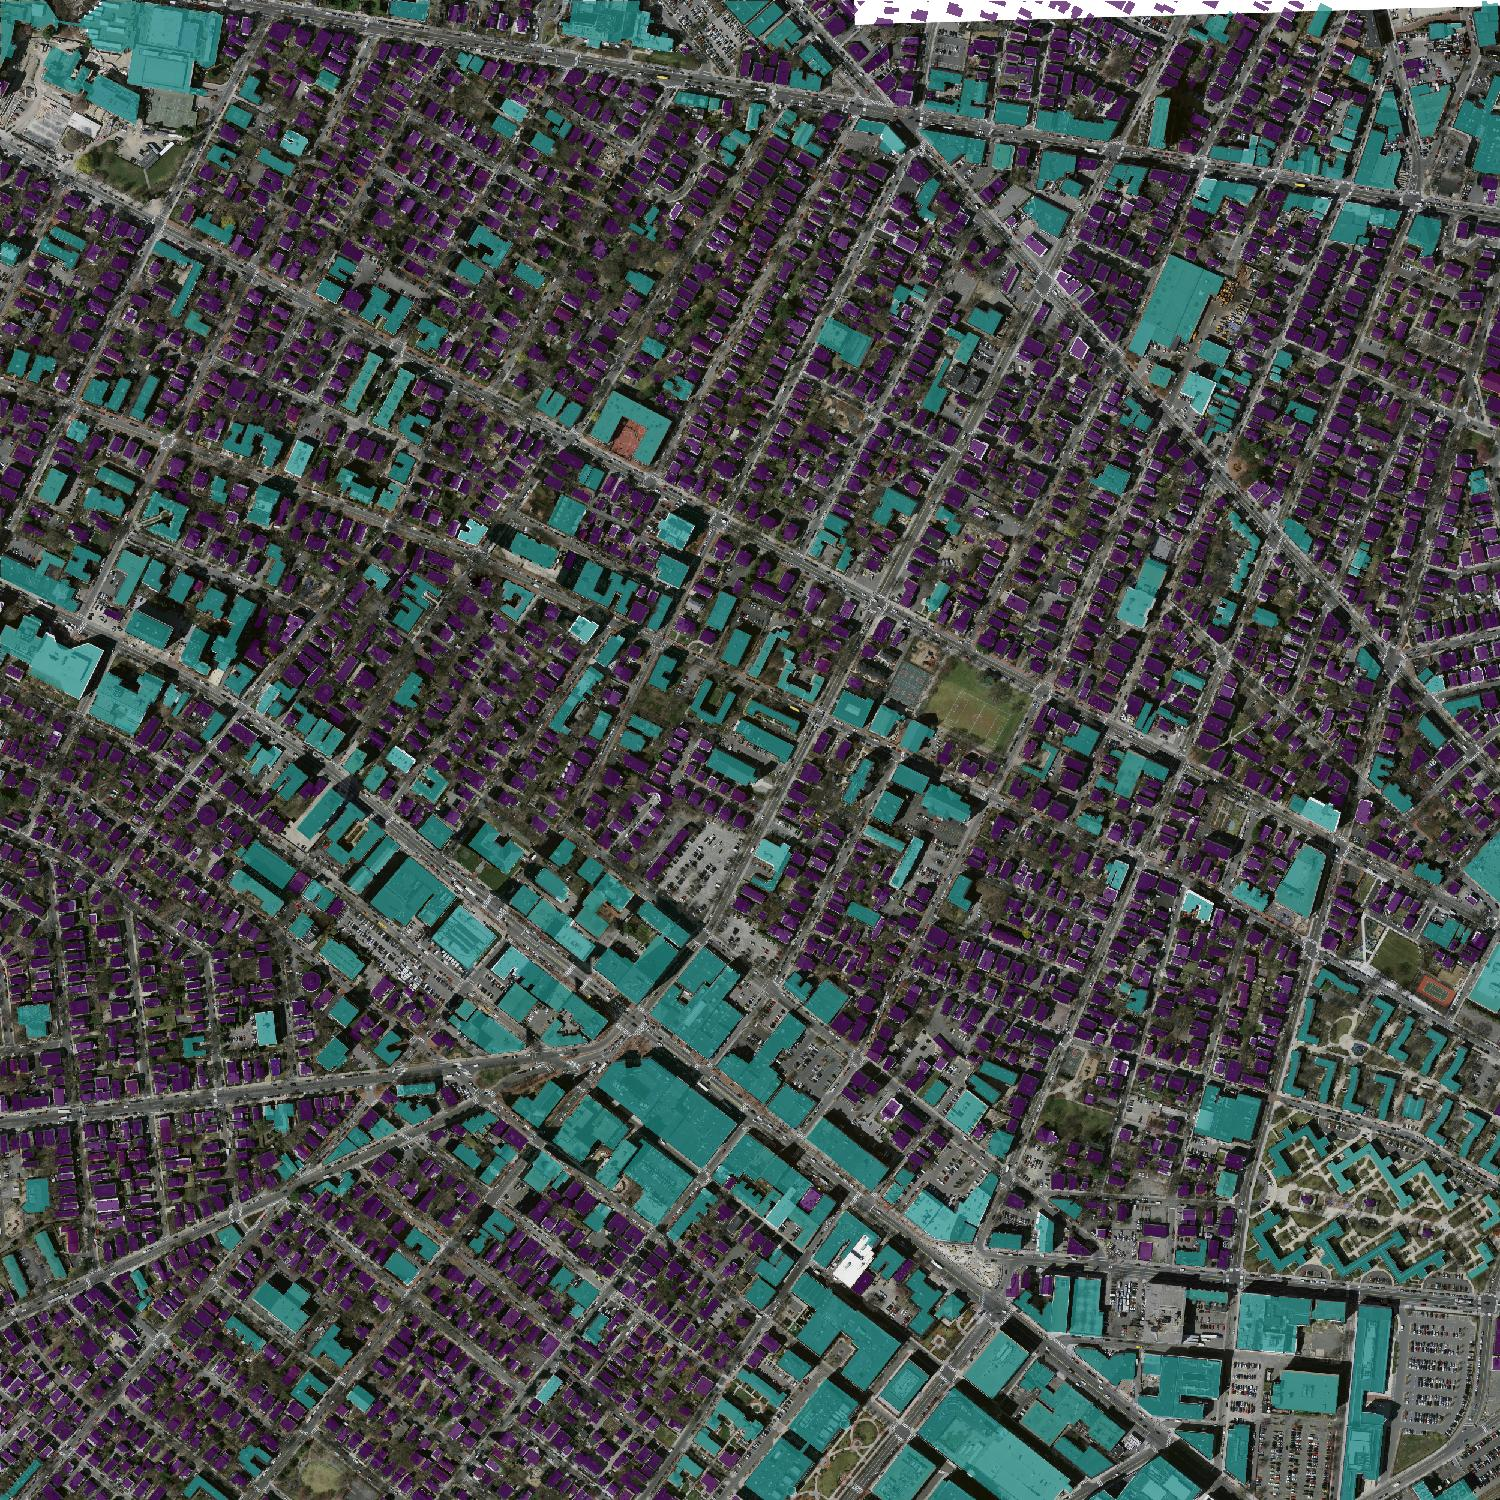
\includegraphics[width=0.25\linewidth]{figures/labelByClass}%
    }
    \hspace{1em}
    \subfloat[Example using an alternative colormap]{%
        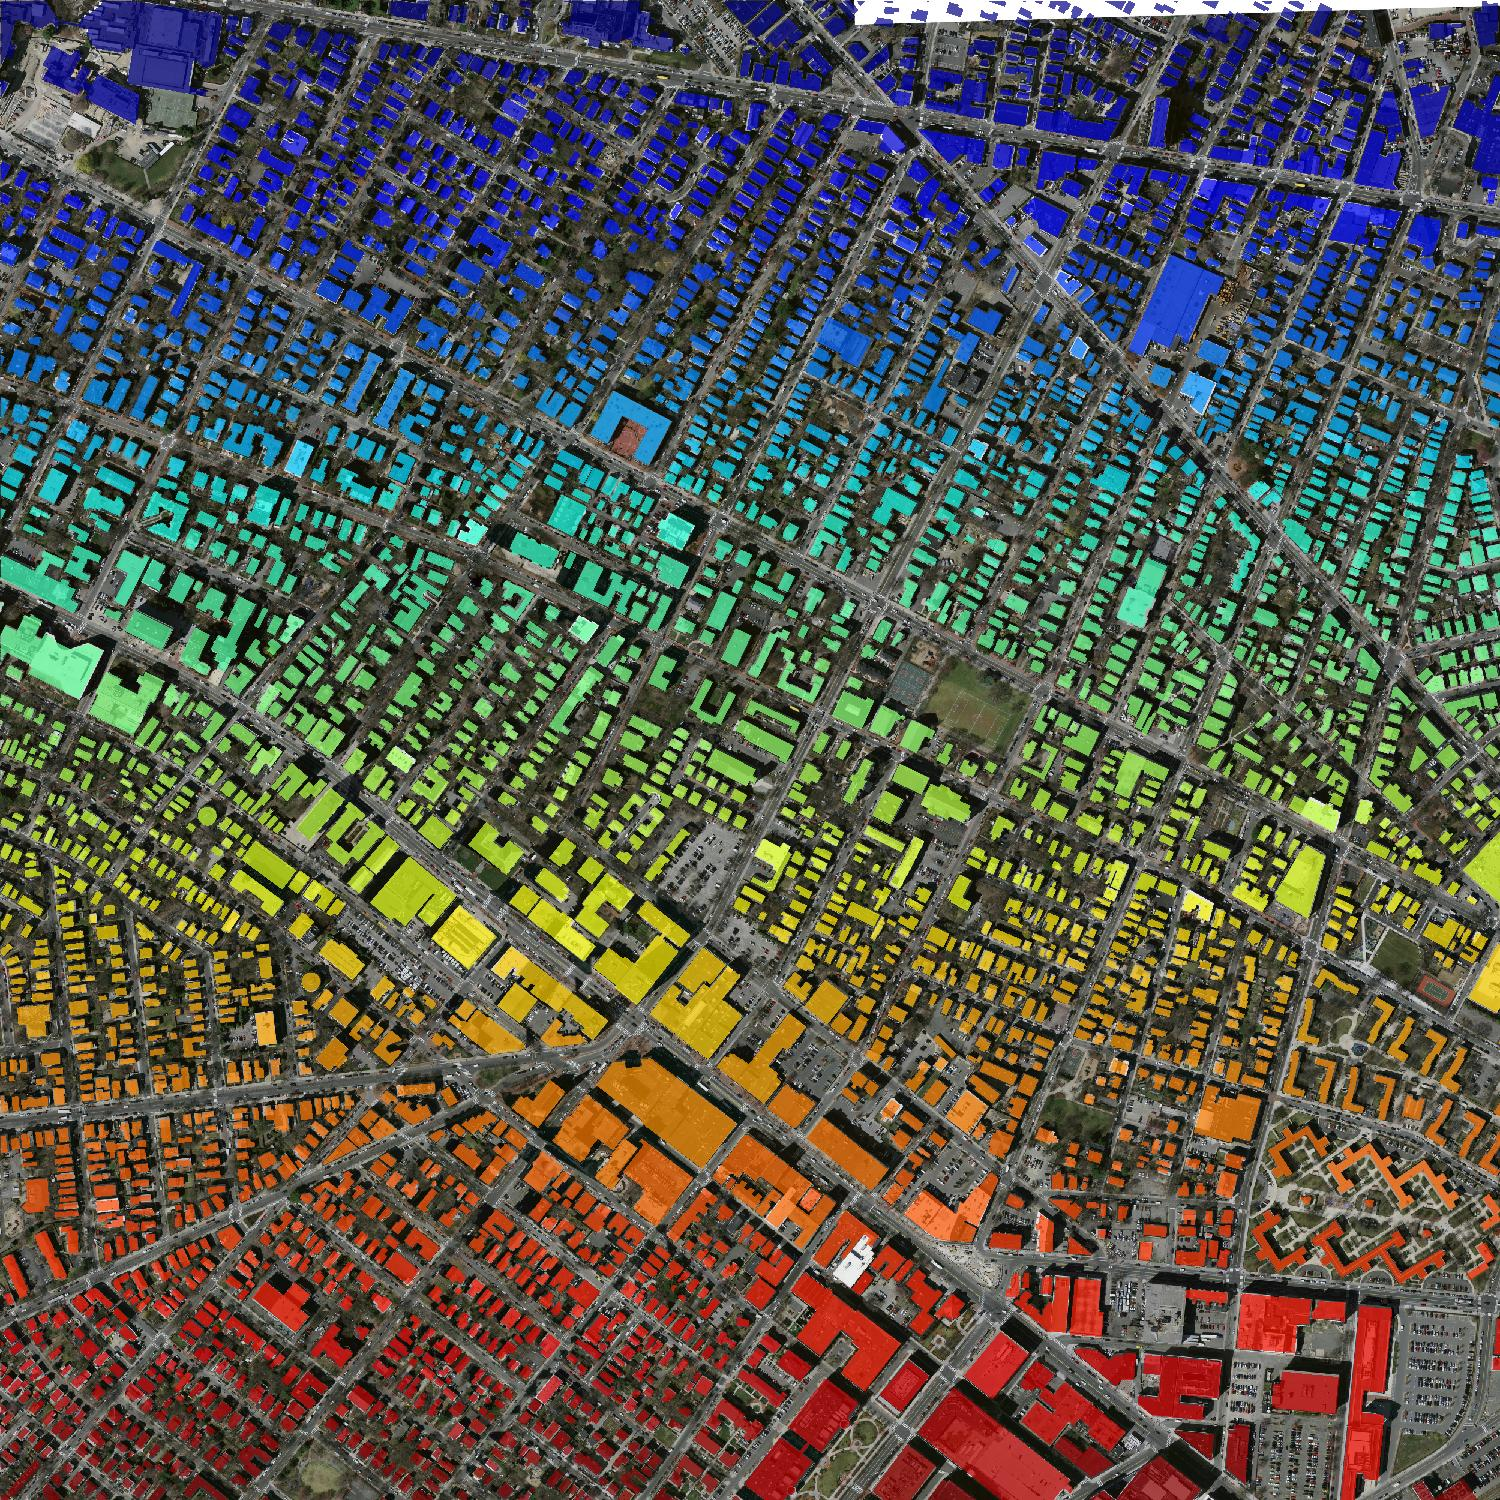
\includegraphics[width=0.25\linewidth]{figures/changeLabelColormap}%
    }
    \hfill
    \caption{Several exports of the same data illustrating the various labeling capabilities within S3A. Arbitrary data columns and arbitrary colormaps may be used.}
    \label{fig:reconfig}
\end{figure*}
}

\newcommand{\makeProcessIllustrationFig}{%
\begin{figure}[!htbp]
    \centering
    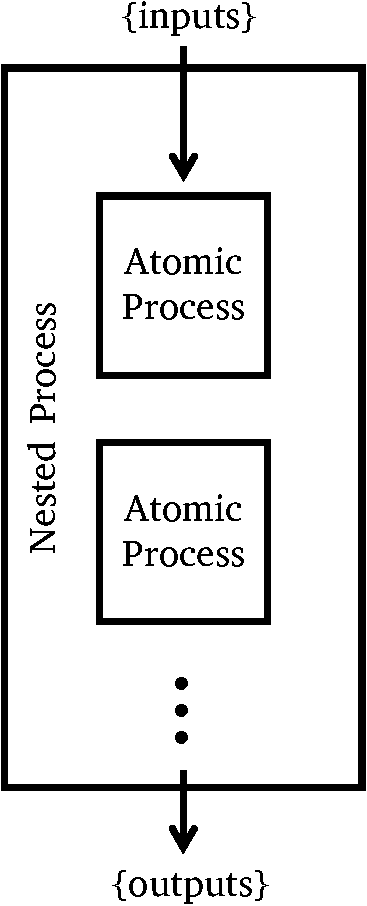
\includegraphics[width=0.3\linewidth]{figures/processIllustration}
    \caption{Depiction of the underlying processing framework. Atomic processes directly wrap functions, and nested processes can contain arbitrary groupings of atomic or nested processes.}
    \label{fig:processIllustration}
\end{figure}
}


\newcommand{\makeAtomicProcFig}{%
\begin{figure*}[!htbp]
    \centering
    \subfloat[Listing for sample outputs]{%
        \RecustomVerbatimEnvironment{Verbatim}{BVerbatim}{}
        \inputminted{Python}{figures/atomicListing.txt}
    }
    \hfill
    \subfloat[Documentation is presented on mouse hover]{%
        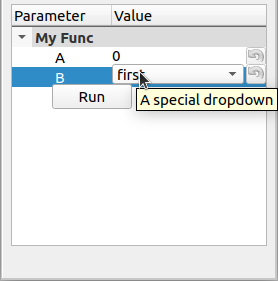
\includegraphics[width=0.29\linewidth]{figures/hoverDoc}%
    }
    \hfill
    \subfloat[GUI constraints are retrieved from specifications]{%
        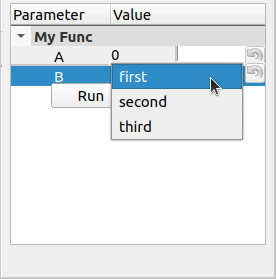
\includegraphics[width=0.29\linewidth]{figures/dropdown}%
    }
    \caption{Several exports of the same data illustrating the various labeling capabilities within S3A. Arbitrary data columns and arbitrary colormaps may be used.}
    \label{fig:atomicProc}
\end{figure*}
}

\newcommand{\makeNestedProcFig}{%
\begin{figure}[!htbp]
    \centering
    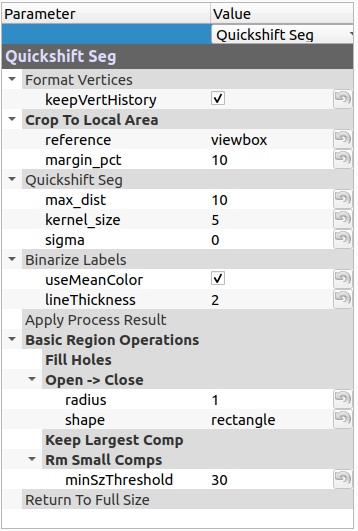
\includegraphics[width=0.5\linewidth]{figures/nestedProc}
    \caption{Processes within S3A can be grouped hierarchically and chained arbitrarily to provide an effective image processing workflow.}
    \label{fig:nestedProc}
\end{figure}
}

\newcommand{\makeAppOverviewFig}{%
\begin{figure*}[!htbp]
    \centering
    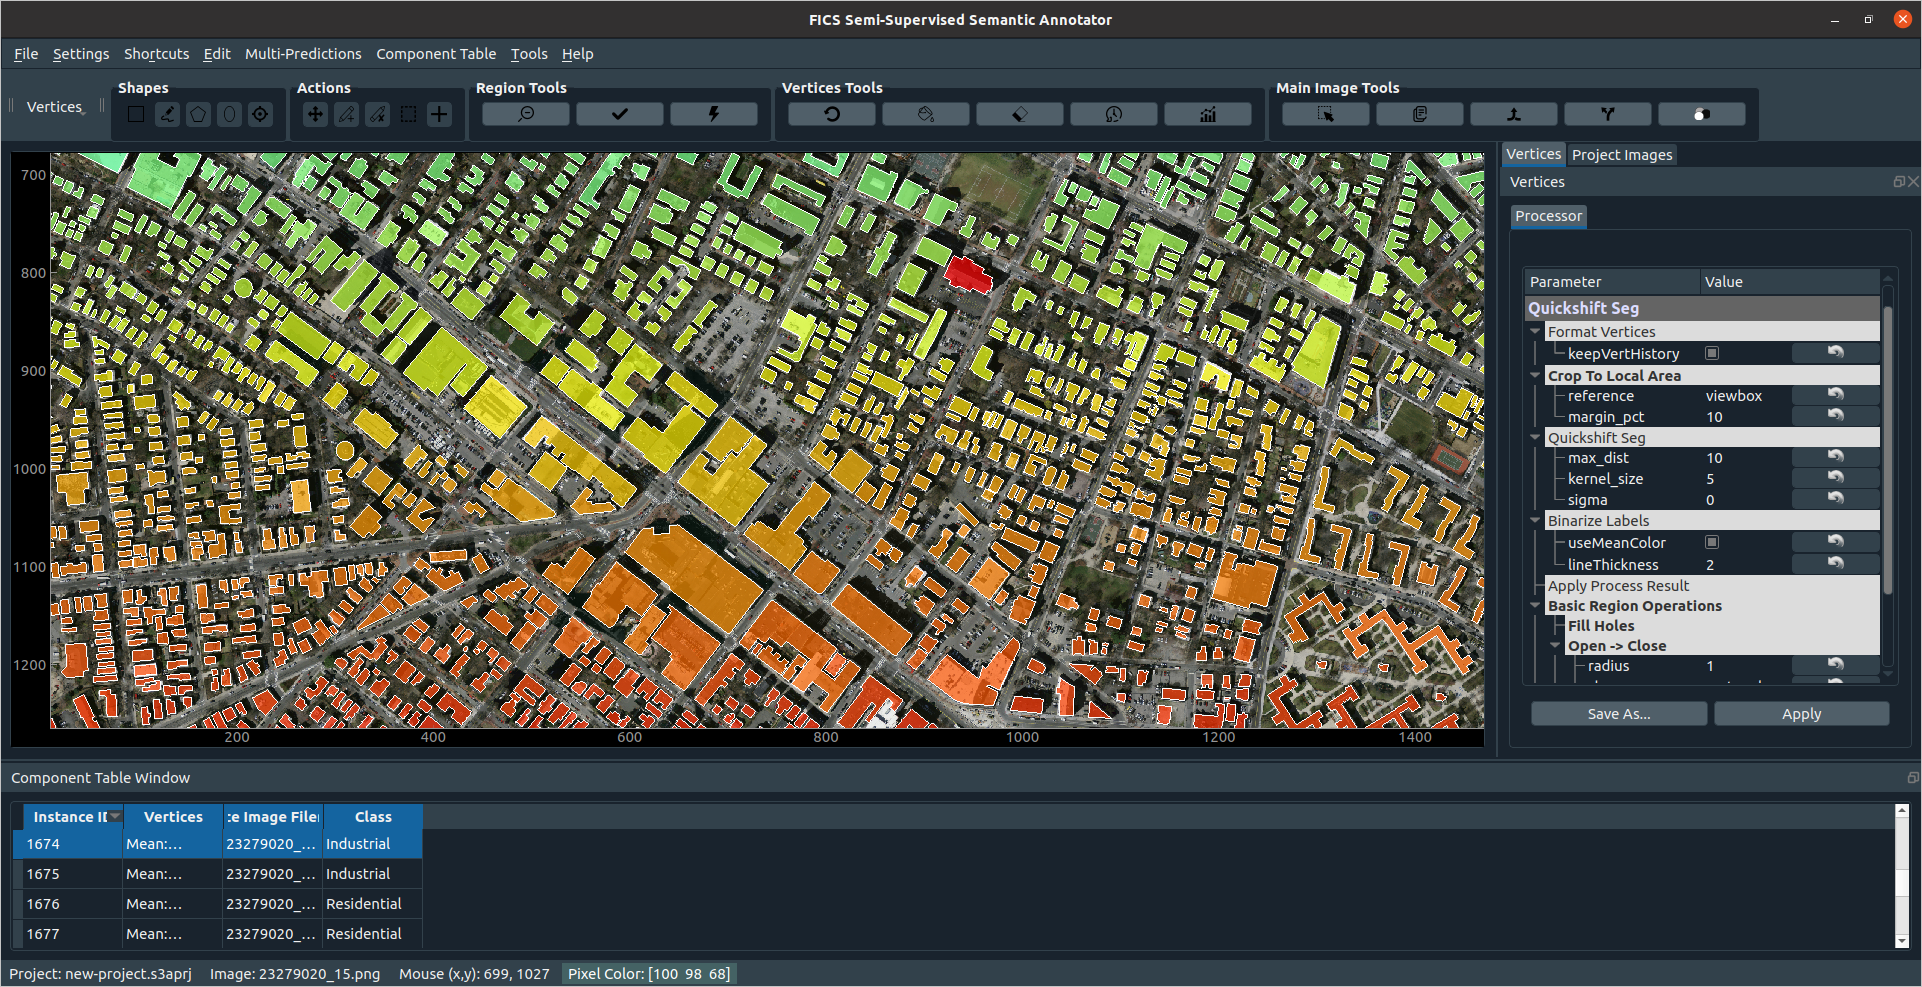
\includegraphics[width=\linewidth]{figures/appOverview}
    \caption{S3A's interface. The main view consists of an image to annotate, a component table of prior annotations, and a toolbar which changes functionality depending on context.}
    \label{fig:appOverview}
\end{figure*}
}

\newcommand{\makeBoundCheckFig}{%
\begin{figure}[!htbp]
    \centering
    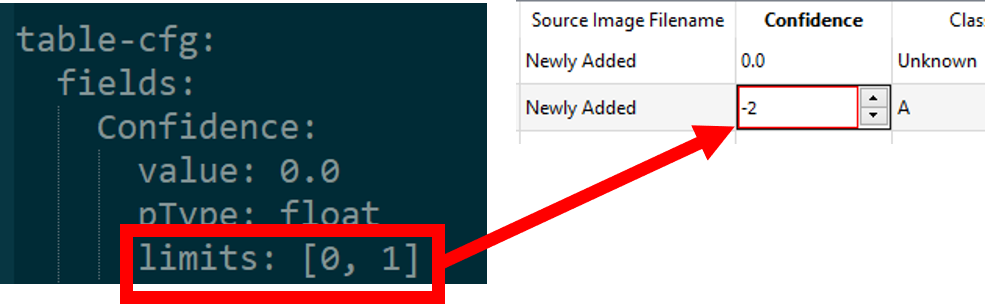
\includegraphics[width=\linewidth]{figures/boundCheck}
    \caption{Automatic bounds checking mean mistakes and highly inaccurate values can be quickly identified before entering a dataset.}
    \label{fig:boundCheck}
\end{figure}
}

\newcommand{\makeStandFilterFig}{%
\begin{figure}[!htbp]
    \centering
    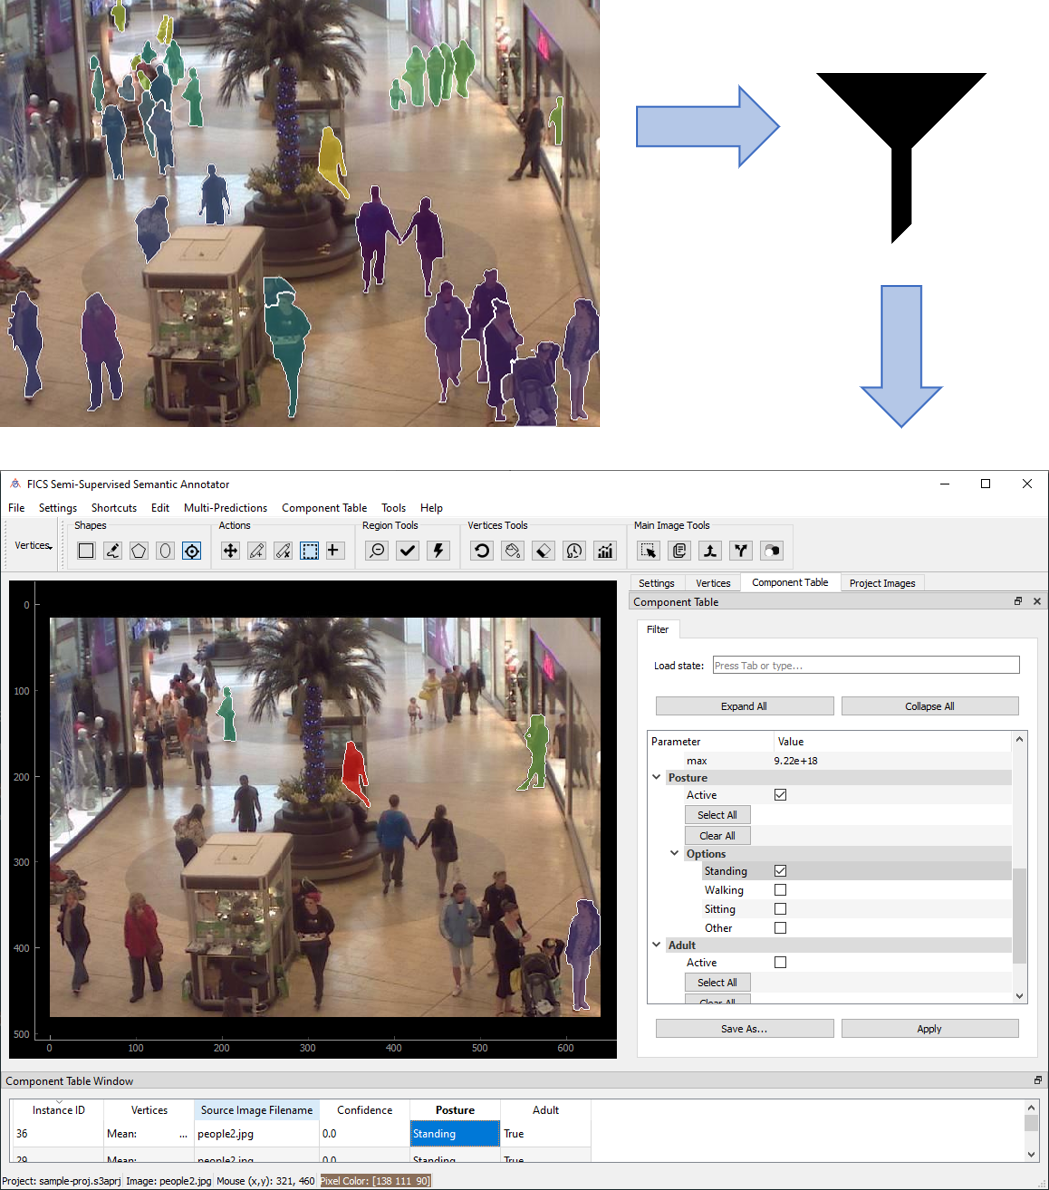
\includegraphics[width=\linewidth]{figures/standFilter_detailed}
    \caption{An active filter for standing people only ensures operators can quickly verify all necessary individuals in the image have been identified. Image under annotation retrieved from \url{https://www.kaggle.com/fmena14/crowd-counting}.}
    \label{fig:standFilter}
\end{figure}
}

\newcommand{\makeCustomMiscFuncFig}{%
\begin{figure*}[!htbp]
    \centering
    \subfloat[Listing for sample outputs]{%
        \RecustomVerbatimEnvironment{Verbatim}{BVerbatim}{}
        \inputminted{Python}{figures/registeredListing.txt}
    }
    \hspace{1em}
    \subfloat[The function can be dynamically called or its inputs modified]{%
        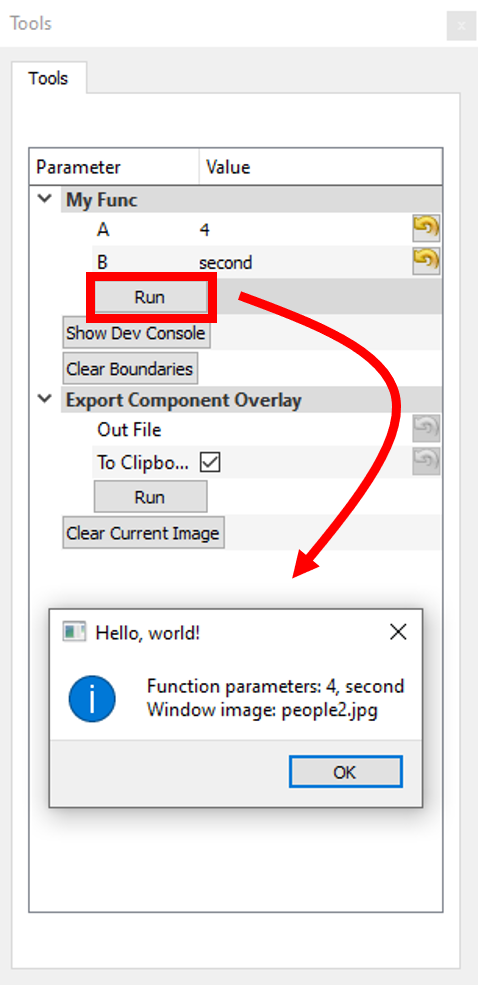
\includegraphics[height=23\baselineskip]{figures/customMiscFunc}%
    }
    \caption{Standalone custom functions can be exposed to the main application in as little as one line of code. A minimal working example (MWE) is shown here.}
    \label{fig:customMiscFuncFig}
\end{figure*}
}

\newcommand{\makeCropExportsFig}{%
\begin{figure}[!htbp]
    \centering
    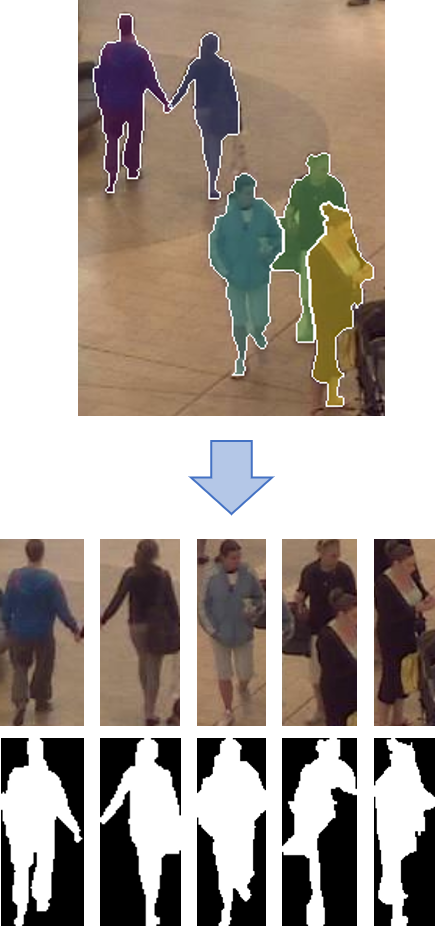
\includegraphics[width=0.5\linewidth]{figures/cropExports}
    \caption{Multiple export formats exist, among which is a utility that crops components out of the image and saves sub-images of their appearance and mask. This is useful for training on multiple forms of machine learning models.}
    \label{fig:cropExports}
\end{figure}
}

\newcommand{\makeRegionAnalyticsFig}{%
\begin{figure*}[!htbp]
    \centering
    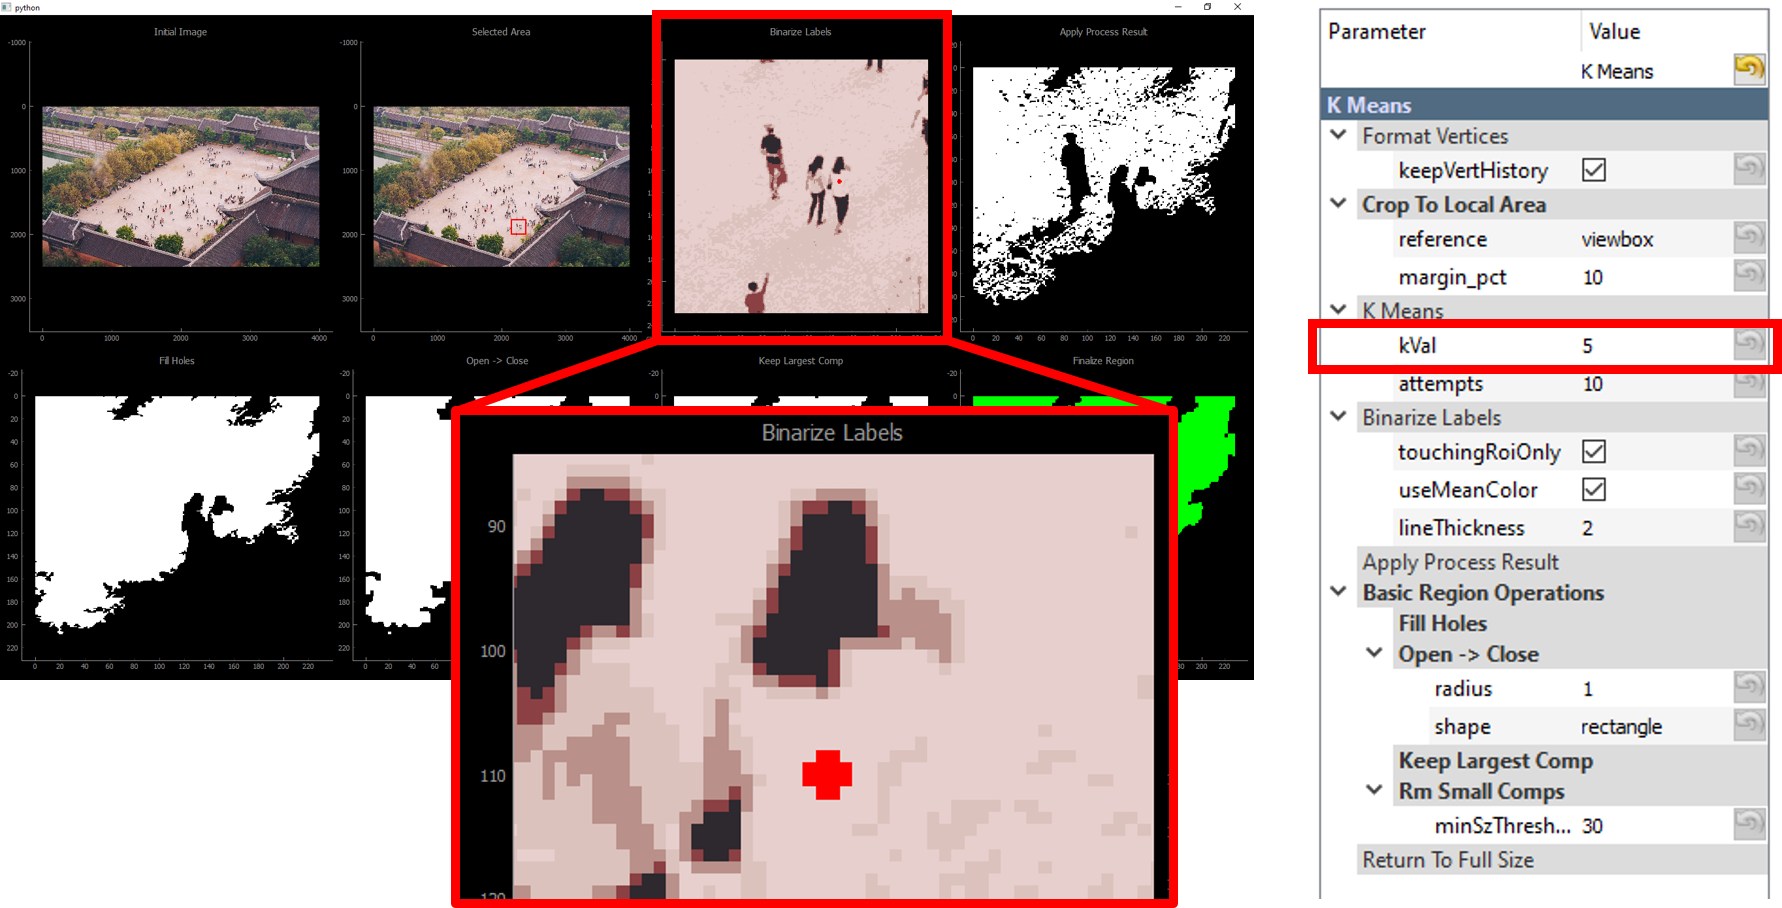
\includegraphics[width=\linewidth]{figures/regionAnalytics}
    \caption{Outputs of each processing stage can be quickly viewed in context after an iteration of annotating. Upon inspecting the results, it is clear the failure point is a low $k$ value during K-means clustering and segmentation. The woman's shirt is not sufficiently distinguishable from the background palette to denote a separate entity. The red dot is an indicator of where the operator clicked during annotation.}
    \label{fig:regionAnalytics}
\end{figure*}
}

\newcommand{\makeSparsePeopleFig}{%
\begin{figure}[!htbp]
    \centering
    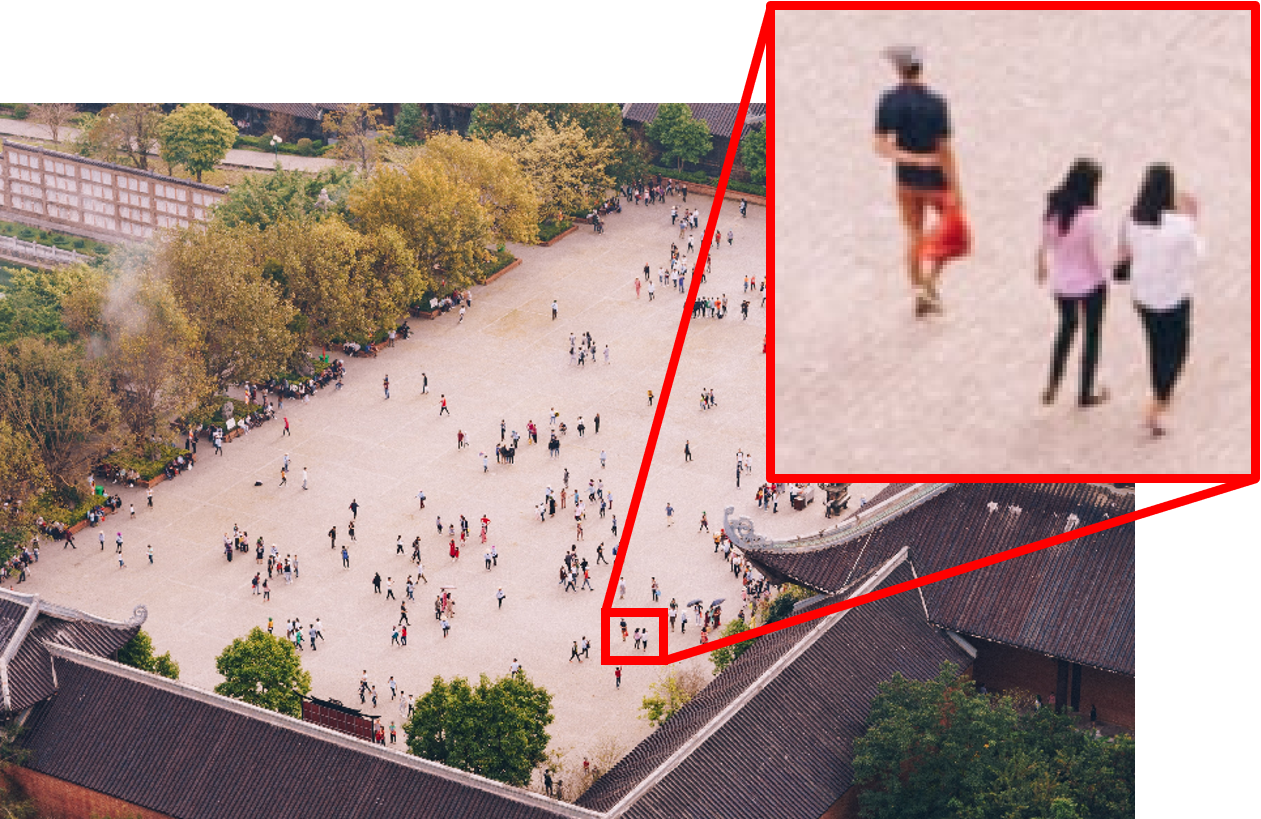
\includegraphics[width=\linewidth]{figures/sparsePeople}
    \caption{Example image where people must be segmented from the background. The low density of foreground pixels means local processing saves orders of magnitudes on some algorithm computation times compared to directly segmenting the entire image. Retrieved from \url{https://unsplash.com/}.}
    \label{fig:sparsePeople}
\end{figure}
}

\newcommand{\makeTemplateMatchFig}{%
\begin{figure}[!htbp]
    \centering
    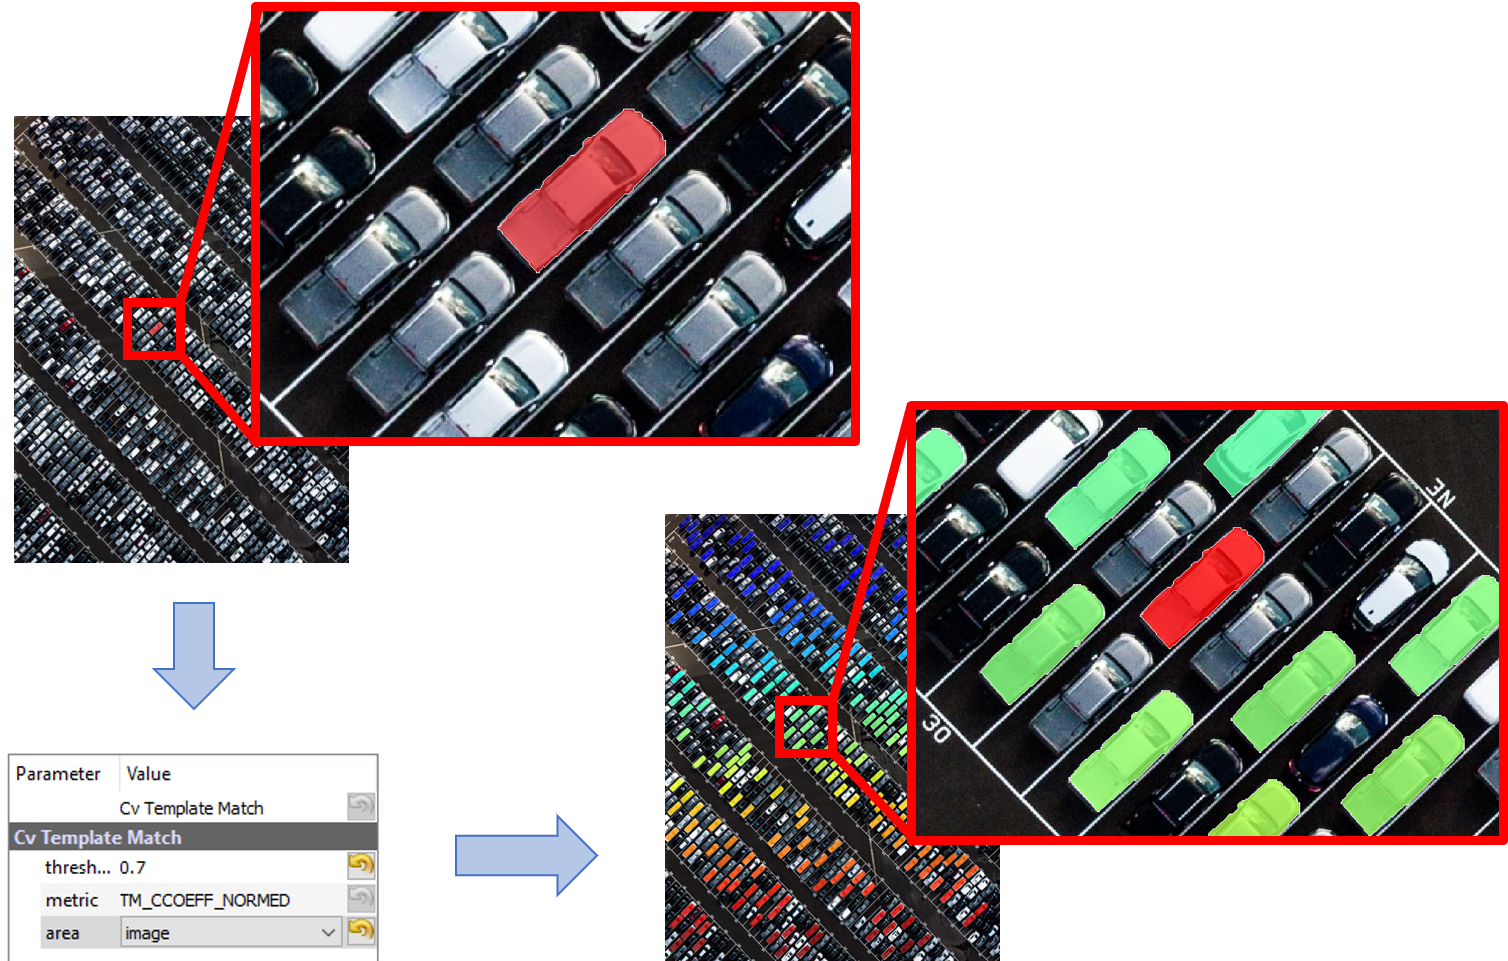
\includegraphics[width=\linewidth]{figures/templateMatch}
    \caption{In cases where repeating structures are prevalent in an image, template matching can be effectively used as a simple region proposal technique. Annotated image retrieved from \url{https://unsplash.com/}.}
    \label{fig:templateMatch}
\end{figure}
}


\newcommand{\makePcbFig}{%
\begin{figure}[!htbp]
    \centering
    \includegraphics[width=\linewidth]{figures/pcb}
    \caption{Example PCB segmentation. Surface-mount device (SMD) properties such as pin count, solder quality, connectivity, and more are difficult or impossible to infer without precise and accurate image segmentation.}
    \label{fig:pcb}
\end{figure}
}